\newif\ifcommentenabled \commentenabledtrue
\newcommand{\TS}[1]{\ifcommentenabled\textcolor{red}{TS: #1}\fi}
\newcommand{\TK}[1]{\ifcommentenabled\textcolor{blue}{TK: #1}\fi}
% TODO: How can I write E-LET like those rules in TaPL?

\documentclass[12pt, a4paper, titlepage]{report}
\usepackage[cache=false]{minted} % highlight programming languages
\usepackage[dvipdfmx]{graphicx}
\usepackage[nottoc,numbib]{tocbibind}
\usepackage[utf8]{inputenc}
\usepackage{amsmath}
\usepackage{amssymb}
\usepackage{color}
\usepackage{enumerate}
\usepackage{hyperref}
\usepackage{bussproofs}
\usepackage{mathptmx}
\usepackage{mathpartir} % automatically fit multiple math expressions
\usepackage{pdfpages} % PDF inclusion
\usepackage{verbatim} % comment environment
\hypersetup{
  colorlinks = true,
  linkcolor = cyan
}

% Title Page
\title{
  Bachelor Thesis \\
  Type- and Sequential Effect-Guided Programming by Example
}
\author{
  03190413 Takemaru Kadoi
  \\[1cm]
  {\small Supervisor: Prof. Masahiro Fujita},
  {\small Advisor: Assistant Prof. Taro Sekiyama}
  \\[1cm]
  {\small University of Tokyo, Department of Information and Communication Engineering}
}
\date{\today}

\begin{document}

% front page
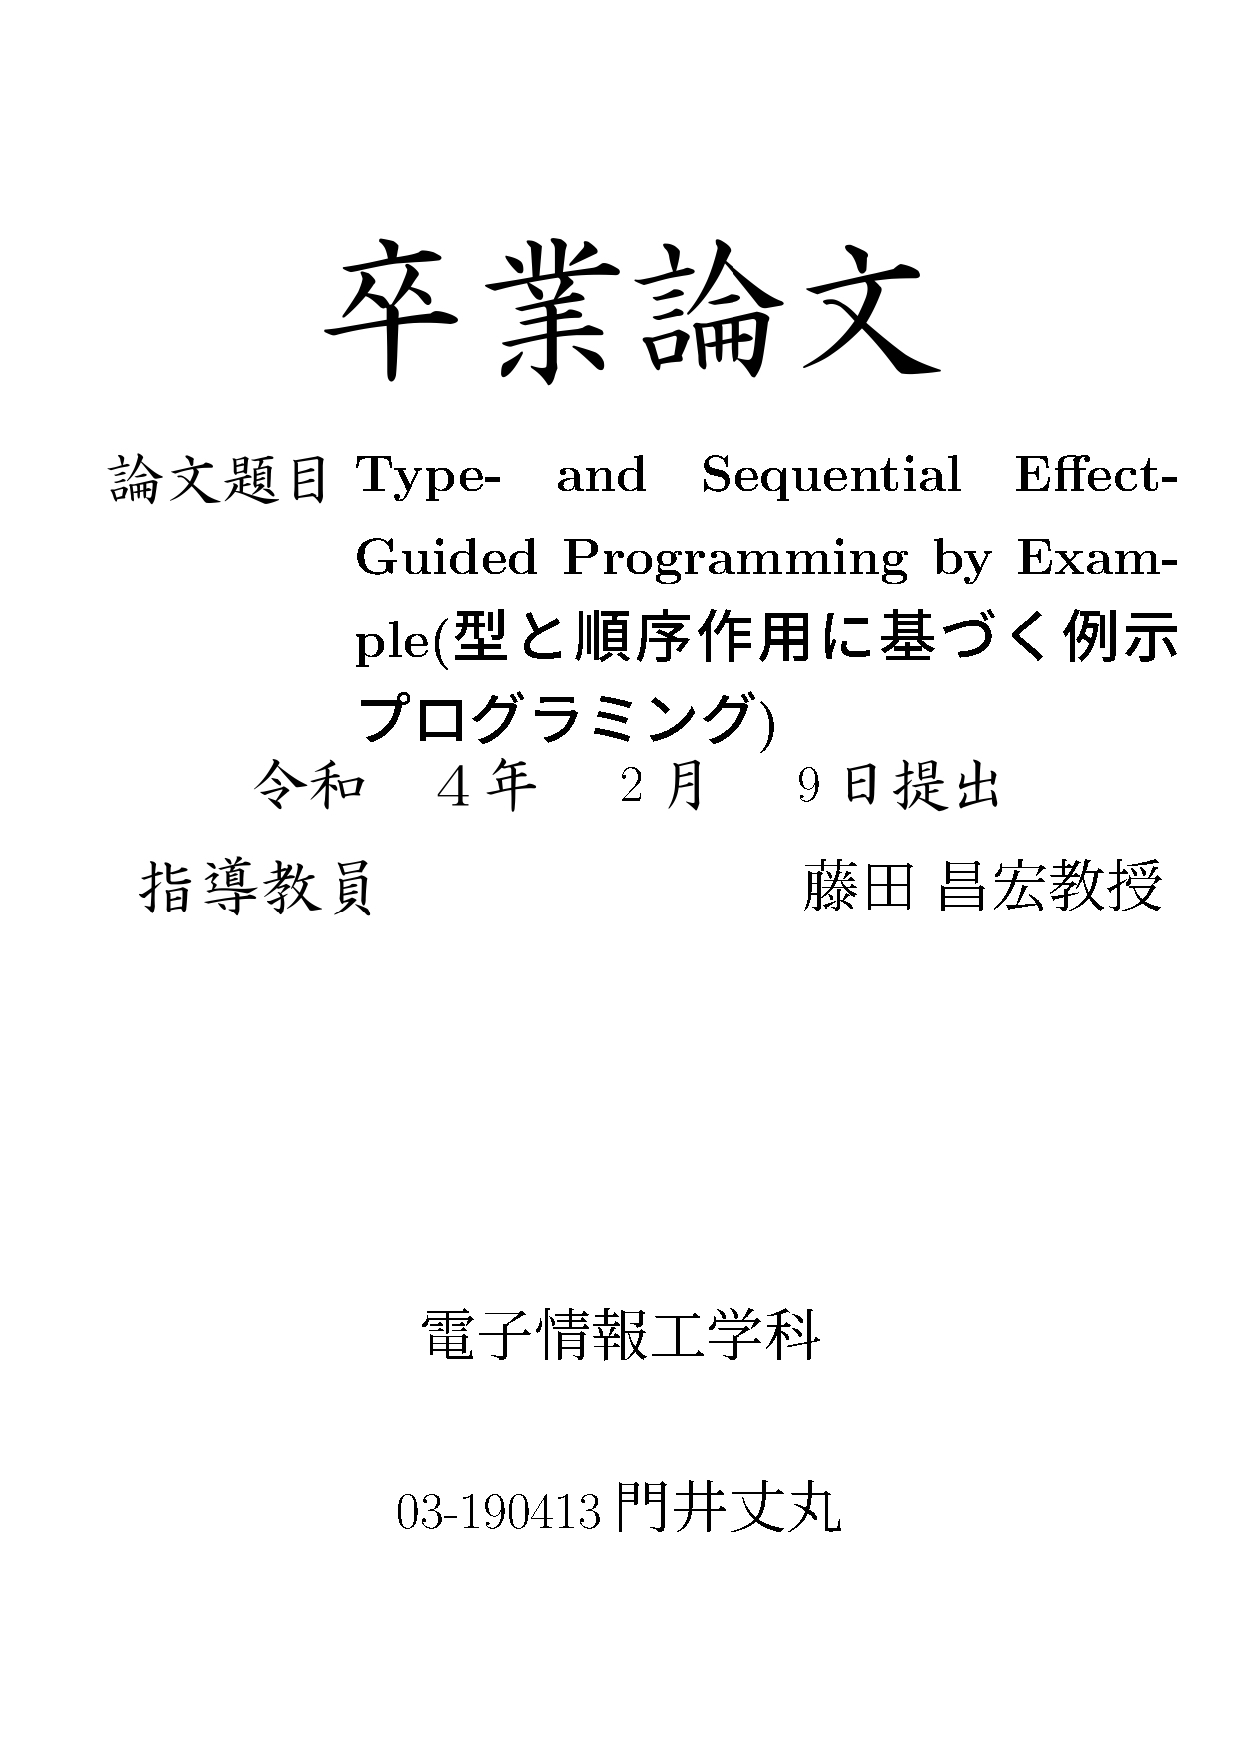
\includepdf[pages={-}]{images/sotsuronFront.pdf}

% header
\maketitle
\newpage
\tableofcontents
\newpage

\chapter*{Acknowledgment}
This research was supervised by Prof. Fujita at the University of Tokyo and supported by Assistant Prof. Sekiyama at National Institute of Technology. \\
I thank my colleagues at the University of Tokyo, Miyasaka-san, Koike-san, Yu-san, Nagasawa-san, and Yi-san.
I also show my gratitude to my good friends,
  \href{https://twitter.com/97sktk}{Saeki},
  \href{https://twitter.com/9SKEgI72RcOWxB8}{haru},
  \href{https://twitter.com/LdCqh1}{Mao Kaneyasu},
  \href{https://twitter.com/NaomiatLibrary}{Naomi},
  \href{https://twitter.com/TaKOBKi}{TaKO8Ki},
  \href{https://twitter.com/Tmstmput}{Tsumiki},
  \href{https://twitter.com/akio_utsuroido}{Akio},
  \href{https://twitter.com/gasukkkgesu}{Gasu},
  \href{https://twitter.com/hamburg_soshun}{Soshun},
  \href{https://twitter.com/macrokoala}{Chen},
  \href{https://twitter.com/nozo_moto}{Nozomi},
  \href{https://twitter.com/readonly_true}{Arahata},
  \href{https://twitter.com/wan__nyan__wan}{hnkz},
  and
  \href{https://twitter.com/cheripori}{Sakura}.

% overview of the research topic
\chapter{Abstract} \label{chapter:abstract}
In recent years, several tools have been developed to enhance the productivity of programmers.
In particular, tools for generating code have attracted a lot of attention, and program synthesis is a research field that supports this development.
Program synthesis requires specifications with which users tell a computer what they want to achieve.
In the case of logical formulae, it is
difficult for programmers who are not skilled in math while its strictness contributes to accurate code generation.
With natural language, computers may not be able to understand the meaning, and the intention may not be conveyed correctly even though programmers can find it easy to write specifications.
This paper examines the use of a type and effect system as a specification that is easy to understand by both humans and computers alike. The types are properties of data and can be used to describe the input and output of a function. The effects, which can explain the internal processes of a function, represent a transition in a state, such as the value of a variable, shared memory between threads, and I/O operations.
Types are familiar to programmers who use statically typed languages.
Many users are unfamiliar with effects, but the effects can describe the internal behavior of programs and are easy to understand if designed properly.
By utilizing type and effect, I can efficiently explore candidate code and demonstrate that the intended code will be generated. I will demonstrate some specifications and an example of a program that has been generated based on these specifications.
\TS{(DONE)How do you synthesize programs with types and effects?  What experiments are (planed to be) conducted?  How about results?} \TK{describe how to synthesize and what to do.}

In Chapter \ref{chapter:introduction}, I discuss the motivation for this research, what program synthesis is, and existing methods  The details of the existing methods can be discussed in the related work chapter, which should be  put before the conclusion.
I give examples of existing researches in Chapter \ref{chapter:relatedWork}.
I explain my proposed method in Chapter \ref{chapter:method}.
I present in Chapter \ref{chapter:experiment} the results obtained by the proposed method and evaluate them.
Chapter \ref{chapter:conclusion} concludes with a summary of the results and evaluation, as well as future issues.

\chapter{Introduction}\label{chapter:introduction}
\TS{Introduction should include a summary of what this thesis achieves.  The details of the existing methods can be discussed in the related work section, which should be  put before the conclusion.} \TK{move "Related Work"(previous "Existing methods") to after this chapter and add section "Achievement" in this chapter}
  \section{Motivation}
    The purpose of this research is to contribute to programming efficiently and safely in the current software-centric world that demands for many lines of secure code.
    I tackle this problem by using a type-effect system and a technique of program synthesis.
    Bodik insists that this issue is tractable from non-programmers' and programmers' perspectives \cite{bodik:2015}.
    I, however, focus only on a programmer point of view.

    % present situation(type is used in everyday development, generating code is required)
    Today, more and more people are developing software.
    Thus, it can be said that an increasing number of people are writing programming languages proportionally.
    Tools to assist programmers are appearing more and more.
    For example, GitHub Copilot based on the research by Chen et al. \cite{Chen:2021} completes source code from function names and comments.
    It is obvious that it uses program synthesis techniques.
    DeepMind has also recently developed AlphaCode \cite{Li:2022}, an AI that can automatically solve competitive programming problems.
    As a result of the current situation, the demand for secure code is also increasing.
    Recent software development is facilitated by programming languages that are based on type systems, such as Rust, TypeScript and Scala.
    This shows that the type theory is not only an interesting but also a practical research topic, and modern programmers are familiar with the notion.
    Additionally, the increasing demand illustrates the need for more time-efficient and productive programming.
    The program synthesis fits for this requirement because it is a research topic to deal with easy code generation.

    % what to do(type is usable to boost efficient programming)
    I am motivated by these trends in my research.
    My goal is to help people develop reliable software easily through the type theory and the program synthesis.
    An additional point that I would like to incorporate into my research is the effect system, which is an informative and descriptive system for programming languages.
    This system allows us to describe the internals of a function, which results in high-quality code generation.
    Namely, we can use the system to generate more secure and intended code than code without it.
    Although this concept is unfamiliar to many programmers, the one in this paper is easily understandable and its popularity is not a big obstacle.

  \section{Program Synthesis}
    In this section, I would like to explain what the program synthesis is for those new to this field.
    Gulwani, Polozov, and Singh summarize it as ``the task of automatically finding a program in the underlying programming language that satisfies the user intent expressed in the form of some specifications'' in their survey paper \emph{``Program Synthesis''} \cite{gulwani:2017}.

    I illustrate the process of the program synthesis below.
    \begin{figure}[htbp]
      \centering
      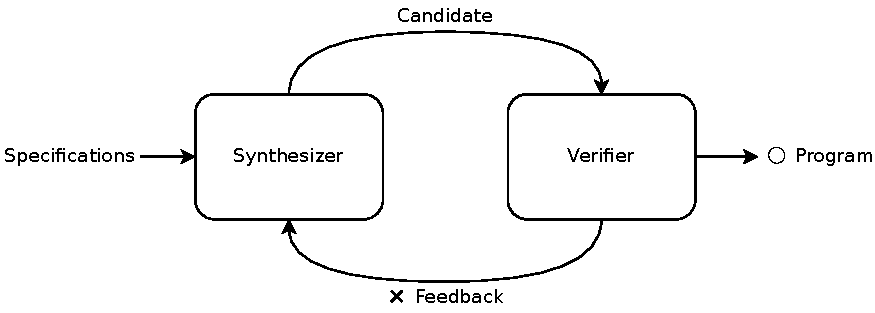
\includegraphics[width=1\textwidth]{images/synthesis.pdf}
      \caption{How the program synthesis generates program}
      \label{synthesisOverview}
    \end{figure}

    The program synthesis consists of 4 steps.
    \begin{enumerate}
      \item To receive specification from a user.
      \item To line up a candidate program.
      \item To check if the candidate program meets some requirements.
      \item To return feedback to the synthesizer or synthesize the program depending on whether it meets the requirements or not
    \end{enumerate}

    Moreover, it has 3 components to consider.
    \begin{enumerate}
      \item User Input
      \item Search Space
      \item Search Technique
    \end{enumerate}
    Synthesizers can accept a variety of inputs.
    Natural languages, logical formulae, and incomplete program code are acceptable forms of communication.
    In relation to the speed and accuracy of program synthesis, search space is a consequential aspect.
    When the target language is a simple language such as brainfuck, which is created by Urban Müller \cite{easter:2020}, the complexity will differ from when the target language is a fully functional language such as C++.
    I have contributed to the field of search technique in this paper.
    The technique is an essential component of the program synthesis process.
    An algorithm determines how fast and how accurately a synthesizer will produce code, and it inseparable from the two factors, user input and search space.

    I am going to deal with these questions in section \ref{section:synthesisProcess}, in which I cover how to synthesize a program.

  \section{Achievement} % contribution of this paper and intro to technical part
  In this research, I have formulated a type and effect system to efficiently synthesize programs by examples.
  By using types and effects, you can synthesize code that would be impossible to synthesize without the use of types and effects due to the explosion of time complexity.

  I defined my own programming language syntax.
  I then defined how that programming language would be evaluated.
  I defined the type and effect system that the programming language should follow to ensure its type safety.
  If a language is mathematically guaranteed to be safe on its runtime, it can be used for large scale software development.
  I have formulated a system for program synthesis targeting this language, using parts of it as specifications.

\chapter{Related Work}\label{chapter:relatedWork}
  The purpose of this chapter is to provide you with a brief overview of existing search techniques that seem to be relevant. As I said in the previous section, one of the factors that have improved the tractability of search space is new search techniques.
  It is pertinent to note that even though I will describe some techniques as separate ones, they are all interconnected. A type of approach is used by another type of approach and vice versa. This categorization is just to clarify what aspects different algorithms have in common.

  \section{Enumerative Search}
  Enumeration is the most efficient way of searching since it overlooks nothing.
  Nevertheless, it has a trade-off.
  The search space is enormous.
  In order to solve in realistic time, you need to prune some candidate programs.
  Several pruning techniques have been developed.
  The basic idea is to enumerate all trees and prune trees equivalent to those already explored.
  I briefly introduce two of them, top-down tree search and bottom-up tree search.
  Top-down tree search starts from the grammar of programming languages, which means that they search nonterminals in terminals.
  On the other hand, bottom-up tree search starts from expressions.

  \section{Constraint Solving}
    Constraint solving is \textit{finding an instantiation of free variables in a formula}. This requires more rigorous specification than other techniques and syntactic program restrictions which are encoded so that you can find true models for a correct program.
    I will give you some explanations about component-based synthesis proposed by Jha et al. \cite{jha:2010}.
    This type of synthesis encodes the language and its spec into SAT/SMT constraints precisely.
    An SMT solver like \textit{Z3} \cite{moura:2008} solves the constraints.
    A component is given in the form of a specification with an input and output pair, which are written as logical formulae.
    In other words, each component is defined as a specialized function.
    Minimum program encoded by these functions has three attributes, which introduced by Jha et al.
    \begin{enumerate}
        \item is well-formed
        \item uses all components without violating their respective specs
        \item is consistent with the provided spec
    \end{enumerate}
    Using these characteristics, Jah et al. produced a complete SMT encoding for the whole program synthesis.

  \section{Stochastic Search}
    Stochastic search is another approach I discuss in this section.
    Stochastic methods use the distribution over the space of programs in the hypothesis space that is conditioned on the specification to obtain a consistent program.
    The learned distribution will lead to a better prediction rate of programs that correspond to the specification.

    Figure \ref{stochastic} is an example of stochastic search.
    Suppose each circle is a candidate of an AST node and each arrow points to the syntactic candidates of the next node with its percentage.
    Stochastic search technique uses the probabilities to determine what code to synthesize.
    The technique uses code base to predict the percentages.
    \textit{STOKE} \cite{Schkufza:2016}, an implementation on program optimization uses stochastic search like this.

    \begin{figure}[htbp]
      \centering
      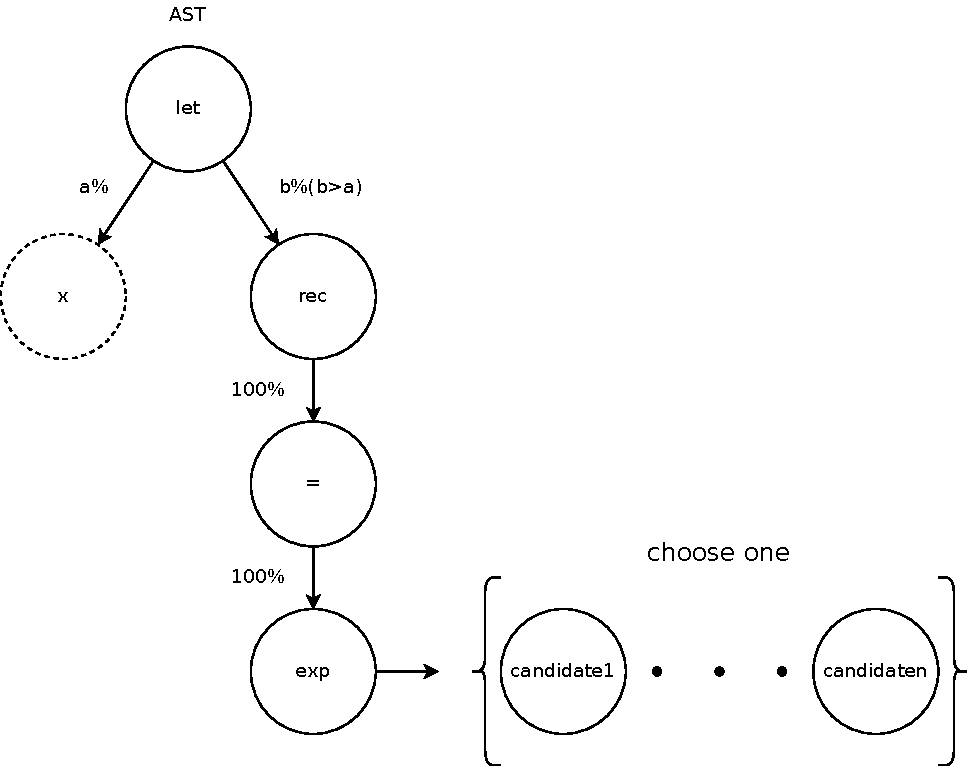
\includegraphics[width=11cm]{images/stochastic.pdf}
      \caption{An example of stochastic search}
      \label{stochastic}
    \end{figure}

    The stochastic Syntax Guided Synthesis (SyGuS) solver uses the Metropolis-Hastings algorithm \cite{alur:2013}.
    We can represent the space of all possible programs in the hypothesis space with a large dense graph.
    Each node is a partial expression and an edge from node $n_1$ (= $e_1$) to node $n_2$ (= $e_2$) signifies that $e_2$ can be obtained from $e_1$.
    Each edge has a probability that $e_1$ becomes $e_2$.
    Metropolis-Hastings algorithm, in a nutshell, updates the probabilities and samples the desired program.

    There are other methods based on probability, such as genetic programming, machine learning, and neural programming.
    Although their solutions are not complete, they are highly efficient if you have quantitative objectives.

  \section{Deduction-Based Programming}
    Deduction-based programming is also called programming by examples (PBE).
    This approach consists of intent specifications, program space, and search algorithms.
    Given input/output examples, a synthesizer generates a candidate program \textbf{P}.
    Using an SMT solver, we efficiently search for a program in the hypothesis space.
    If the verifier finds a counter-example, sends the synthesizer feedback \textbf{F}.
    Given a new input/output example, the synthesizer will produce another candidate until the \textbf{P} is verified.

    This technology is also used in Excel, which is commonly used around the world.
    The technology of transforming the text of an Excel cell is based on Gulwani's research called Flash Fill\cite{gulwani:2011}.
    This research, which creates appropriate cells from input and output examples, connects the results of academia to make them available to end users, and won the Most Influential POPL Paper Award.
    Polozov and Gulwani also presented FlashMeta\cite{polozov:2015}, a framework for PBE that can achieve Flash Fill-like results by simply defining DSLs.
    This technology is expected to make PBE more widely used in the future.


  % TODO: add \section{type-driven program synthesis}

% my approach to the problem
\chapter{Method}\label{chapter:method}
  In this chapter, I am going to introduce the internals of $\mathbf{Titan}$, which is a programming language and a tool for program synthesis.
  First, I will introduce its syntax, and next its semantics.
  After that, I will explain you how to synthesize Titan from its specifications.
  Rules in this chapter are inspired by a textbook \emph{"Types and Programming Languages"} \cite{pierce:2002} and a paper \emph{"RbSyn: Type- and Effect-Guided Program Synthesis"} \cite{guria:2021}.
  \section{Syntax}
    Figure \ref{fig:syntax} shows the syntax of $\mathbf{Titan}$.
    $\mathbf{Titan}$'s components can be divided into values, expressions, unary operators, binary operators, types, effects, an type environment, an effect environment.
    $\mathtt{v}$ is values. It consists of boolean, integer, string, and unit, which is the same as nothing.
    $\mathtt{e}$ is expressions. Every expression is evaluated to values. An expression can be a value, a variable, a unary operator and it operand, a binary operator and its operands, an expression application, an if expression, a let expression, a function expression, a type hole, an effect hole, a file-read, or a file-write.
    Unary Operators $\mathtt{uop}$ and binary operators $\mathtt{bop}$ works with operands as in other programming languages.
    $\mathtt{\tau}$ has 6 types. boolean, integer, string, unit(do nothing), any, and type-to-type.
    $\mathtt{\epsilon}$ has 7 effects. Effects related to I/O, a do-nothing effect, an \textit{any} effect, and an effect-to-effect effect.
    $\mathtt{\Gamma}$ and $\mathtt{E}$ links identifiers to its type or effect.

    \begin{figure}[htbp]
      \begin{flushleft}
        \textbf{Syntax}
      \end{flushleft}
      \[
      \centering
      \begin{array}{lccl}
        \emph{Values} &
          \mathtt{v} & ::= & \mathtt{boolean \mid integer \mid string \mid unit}\\
        \emph{Expressions} &
          \mathtt{e} & ::= & \mathtt{v} \mid \mathtt{x} \mid \mathtt{uop\ e \mid e\ bop\ e} \\
          & & \mid & \mathtt{e\ e} \\
          & & \mid & \mathtt{if}\ \mathtt{b}\ \mathtt{then}\ \mathtt{e}\ \mathtt{else}\ \mathtt{e} \\
          & & \mid & \mathtt{let}\ \mathtt{x = e}\ \mathtt{in}\ \mathtt{e} \\
          & & \mid & \mathtt{fun}\ \mathtt{(x : \tau) : \tau\ "\{"\ \{\epsilon\}^{+}\ "\}" \to e} \\
          & & \mid & \mathtt{hole : \tau} \\
          & & \mid & \mathtt{hole : "\{" \{\epsilon\}^{+} "\}"} \\
          & & \mid & \mathtt{fread(e)} \\
          & & \mid & \mathtt{fwrite(e)} \\
        \emph{Unary Operators} &
          \mathtt{uop} & ::= & ! \mid - \\
        \emph{Binary Operators} &
          \mathtt{bop} & ::= & \mathtt{+} \mid \mathtt{-} \mid \mathtt{\times} \mid \mathtt{/} \mid \mathtt{\%} \\
          & & \mid & \mathtt{=} \mid \mathtt{\neq} \mid \mathtt{<} \mid \mathtt{\leq} \\
          & & \mid & \mathtt{>} \mid \mathtt{\geq} \mid \mathtt{\land} \mid \mathtt{\lor} \\
        \emph{Types} &
          \mathtt{\tau} & ::= & \mathtt{\tau_{bool} \mid \tau_{int} \mid \tau_{string} \mid \tau_{unit}} \\
          & & \mid & \mathtt{\tau_{any} \mid \tau \to \tau} \\
        \emph{Effects} &
          \mathtt{\epsilon} & ::= & \mathtt{\epsilon_{open} \mid \epsilon_{read} \mid \epsilon_{write} \mid \epsilon_{close}} \\
          & & \mid & \mathtt{\epsilon_{unit} \mid \epsilon_{any} \mid \epsilon \to \epsilon} \\
        \emph{Type Environment} &
          \mathtt{\Gamma} & ::= & \mathtt{\varnothing \mid x : \tau, \Gamma} \\
        \emph{Effect Environment} &
          \mathtt{E} & ::= & \mathtt{\varnothing \mid x : \epsilon, E} \\
      \end{array}
      \]
      \[
        x \in \textrm{variables}
      \]
      \caption{Syntax of $\mathbf{Titan}$}
      \label{fig:syntax}
    \end{figure}

  \section{Semantics}
    \subsection{Evaluation Rules}
      % TODO: add explanation in the natural language
      Figure \ref{fig:evalRules} shows the evaluation rules of $\mathbf{Titan}$.
      \begin{figure}[htbp]
        \begin{flushleft}
          \textbf{Evaluation Rules} \quad \framebox{$\mathtt{t \to t'}$}
        \end{flushleft}
        \centering
        \begin{mathpar}
          % let
          \dfrac
            {\mathtt{t_1 \longrightarrow t_1'}}
            {\mathtt{let\ x=t_1\ in\ t_2 \longrightarrow let\ x=t_1'\ in\ t_2}}
            \left(\textrm{E-LET}\right) \and
          % if
          \dfrac
            {}
            {\mathtt{if\ true\ then\ t_2\ else\ t_3 \longrightarrow t_2}}
            \left(\textrm{E-IFTRUE}\right) \and
          \dfrac
            {}
            {\mathtt{if\ false\ then\ t_2\ else\ t_3 \longrightarrow t_3}}
            \left(\textrm{E-IFFALSE}\right) \and
          \dfrac
            {\mathtt{t_1 \longrightarrow t_1'}}
            {\mathtt{if\ t_1\ then\ t_2\ else\ t_3 \longrightarrow if\ t_1'\ then\ t_2\ else\ t_3}}
            \left(\textrm{E-IF}\right) \and
          % fun
          \dfrac
            {\mathtt{t_1 \longrightarrow t_1'}}
            {\mathtt{t_1\ t_2 \longrightarrow t_1'\ t_2}}
            \left(\textrm{E-APP1}\right) \and
          \dfrac
            {\mathtt{t_2 \longrightarrow t_2'}}
            {\mathtt{t_1\ t_2 \longrightarrow t_1\ t_2'}}
            \left(\textrm{E-APP2}\right) \and
          \dfrac
            {}
            {\mathtt{(fun\ x \to t_{12}) v_2 \longrightarrow [x \mapsto v_2]t_{12}}}
            \left(\textrm{E-APPABS}\right) \and
          % I/O
          \dfrac
            {\mathtt{t}}
            {\mathtt{fread(t) \longrightarrow string}}
            \left(\textrm{E-READ}\right) \and
          \dfrac
            {\mathtt{t}}
            {\mathtt{fwrite(t) \longrightarrow unit}}
            \left(\textrm{E-WRITE}\right) \and
          % hole
          \dfrac
            {}
            {\mathtt{hole \longrightarrow unit}}
            \left(\textrm{E-HOLE}\right) \and
        \end{mathpar}
        \caption{Evaluation Rules of $\mathbf{Titan}$}
        \label{fig:evalRules}
      \end{figure}

    \subsection{Type/Effect System}
      % TODO: add explanation in the natural language
      Figure \ref{fig:typeEffectSystem} shows the type/effect system of $\mathbf{Titan}$.
      \begin{figure}[htbp]
        \begin{flushleft}
          \textbf{Type/Effect System} \quad \framebox{$\mathtt{\Gamma, E} \vdash \mathtt{t : \tau, \epsilon}$}
        \end{flushleft}
        \centering
        \begin{mathpar}
          % var
          \dfrac
            {\mathtt{x : \tau, \epsilon \in \Gamma, E}}
            {\mathtt{\Gamma, E \vdash x : \tau, \epsilon}}
            \left(\textrm{T-VAR}\right) \and
          % let
          \dfrac
            {\mathtt{\Gamma, E\ \vdash\ t_1 : \tau_1, \epsilon_1 \quad \Gamma, E \vdash x : \tau_1\ \vdash\ t_2 : \tau_2, \epsilon_2}}
            {\mathtt{\Gamma, E\ \vdash\ let\ x=t_1\ in\ t_2 : \tau_2, \epsilon_2}}
            \left(\textrm{T-LET}\right) \and
          % if
          \dfrac
            {}
            {\mathtt{true : \tau_{bool}}}
            \left(\textrm{T-TRUE}\right) \and
          \dfrac
            {}
            {\mathtt{false : \tau_{bool}}}
            \left(\textrm{T-FALSE}\right) \and
          \dfrac
            {\mathtt{\Gamma \vdash t_1 : bool \quad \Gamma, E \vdash t_2 : \tau, \epsilon \quad \Gamma, E \vdash t_3 : \tau, \epsilon}}
            {\mathtt{if\ t_1\ then\ t_2\ else\ t_3 : \tau, \epsilon}}
            \left(\textrm{T-IF}\right) \and
          % fun
          \dfrac
            {\mathtt{\Gamma, x : \tau_1, E, x : \epsilon_1 \vdash t_2 : \tau_2, \epsilon_2}}
            {\mathtt{\Gamma \vdash fun\ (x : \tau_1, \epsilon_1 \to t_2) : \tau_1, \epsilon_1 \to \tau_2, \epsilon_2}}
            \left(\textrm{T-ABS}\right) \and
          \dfrac
            {\mathtt{\Gamma, E \vdash t_1 : \tau_{11}, \epsilon_{11} \to \tau_{12}, \epsilon_{12} \quad \Gamma, E \vdash t_2 : \tau_{11}, \epsilon_{11}}}
            {\mathtt{\Gamma, E \vdash t_1\ t_2 : \tau_{12}, \epsilon_{12}}}
            \left(\textrm{T-APP}\right) \and
          % I/O
          \dfrac
            {\mathtt{\Gamma \vdash t_1 : \tau_{string}}}
            {\mathtt{\Gamma, E \vdash fread(t_1) : \epsilon_{open} \to \epsilon_{read} \to \epsilon_{close} \longrightarrow t_2 : \tau_{string}}}
            \left(\textrm{T-READ}\right) \and
          \dfrac
            {\mathtt{\Gamma \vdash t_1 : \{\tau_{bool}, \tau_{int}, \tau_{string}\}}}
            {\mathtt{\Gamma, E \vdash fwrite(t_1) : \epsilon_{open} \to \epsilon_{write} \to \epsilon_{close} \longrightarrow t_2 : \tau_{unit}}}
            \left(\textrm{T-WRITE}\right) \and
          % hole
            \dfrac
              {}
              {\mathtt{hole : \tau_{unit} \longrightarrow unit : \tau_{unit}}}
              \left(\textrm{T-HOLET}\right) \and
            \dfrac
              {}
              {\mathtt{hole : \epsilon_{unit} \longrightarrow unit : \epsilon_{unit}}}
              \left(\textrm{T-HOLEE}\right) \and
        \end{mathpar}
        \caption{Type/Effect System of $\mathbf{Titan}$}
        \label{fig:typeEffectSystem}
      \end{figure}

  \section{Synthesis Process}\label{section:synthesisProcess}
    % TODO: add explanation in the natural language
    Figure \ref{fig:synthesisRules} shows the synthesis rules of $\mathbf{Titan}$.
    \begin{figure}[htbp]
      \begin{flushleft}
        \textbf{Synthesis Rules} \quad \framebox{$\mathtt{\Gamma, E \vdash t :\tau, \epsilon}$}
      \end{flushleft}
      \centering
      \begin{mathpar}
        % bool
        \dfrac
          {\mathtt{\Gamma \vdash hole : \tau_{bool}}}
          {\mathtt{hole \longrightarrow boolean}}
          \left(\textrm{S-BOOLHOLE}\right) \and
        % int
        \dfrac
          {\mathtt{\Gamma \vdash hole : \tau_{integer}}}
          {\mathtt{hole \longrightarrow integer}}
          \left(\textrm{S-INTHOLE}\right) \and
        % string
        \dfrac
          {\mathtt{\Gamma \vdash hole : \tau_{string}}}
          {\mathtt{hole \longrightarrow string}}
          \left(\textrm{S-STRINGHOLE}\right) \and
        % I/O
        \dfrac
          {\mathtt{\Gamma \vdash t : \tau_{int} \quad E \vdash hole : \epsilon_{open} \to \epsilon_{write} \to \epsilon_{close}}}
          {\mathtt{t\ hole \longrightarrow fwrite(t)}}
          \left(\textrm{S-READ}\right) \and
        \dfrac
          {\mathtt{\Gamma \vdash t : \tau_{bool} \quad E \vdash hole : \epsilon_{open} \to \epsilon_{write} \to \epsilon_{close}}}
          {\mathtt{t\ hole \longrightarrow fwrite(t)}}
          \left(\textrm{S-BOOLWRITE}\right) \and
        \dfrac
          {\mathtt{\Gamma \vdash t : \tau_{int} \quad E \vdash hole : \epsilon_{open} \to \epsilon_{write} \to \epsilon_{close}}}
          {\mathtt{t\ hole \longrightarrow fwrite(t)}}
          \left(\textrm{S-INTWRITE}\right) \and
        \dfrac
          {\mathtt{\Gamma \vdash t : \tau_{string} \quad E \vdash hole : \epsilon_{open} \to \epsilon_{write} \to \epsilon_{close}}}
          {\mathtt{t\ hole \longrightarrow fwrite(t)}}
          \left(\textrm{S-STRINGWRITE}\right) \and
      \end{mathpar}
      \caption{Synthesis Rules of $\mathbf{Titan}$}
      \label{fig:synthesisRules}
    \end{figure}

% my approach to the problem
\chapter{Experiment}\label{chapter:experiment}
  % TODO: situation
    \begin{minted}[breaklines, linenos]{ocaml}
      let _ = print_endline "hello world"
    \end{minted}
  \section{Result}
  % TODO: code generation examples
  \section{Consideration}
  % TODO: what to do

% qualitative result and remaining problems/future work
\chapter{Conclusion}\label{chapter:conclusion}
% TODO: summary of my work
% TODO: qualitative result
% TODO: remaining problems/future work

\bibliographystyle{unsrt}
\bibliography{
  bib/papers,
  bib/textbooks,
}

\end{document}
